% Notwendige Einstellung
  % Tools->Global Options-> Sweave: Weave Rnw files using: knitr
  %                                 Typeset LaTeX into PDF using: pdfLaTeX
  
% Anleitungen: 
  % beamer-Dokumente: http://web.mit.edu/rsi/www/pdfs/beamer-tutorial.pdf
  % Sweave: https://rstudio-pubs-static.s3.amazonaws.com/188117_29a7a382c1884bd98ff54b9c7805613f.html
 
  
%Tell R RStudio the path to latex // put behind "%" before "Compile PDF"
  %If you want RStudio to remember this command each time you start RStudio, you have to add the command to your .Rprofile file.
%Sys.setenv(PATH = paste(Sys.getenv("PATH"), "C:\\Program Files\\MiKTeX 2.9\\miktex\\bin\\x64", sep=.Platform$path.sep))
%Sys.setenv(PATH = paste(Sys.getenv("PATH"), "C:\\Users\\simon/AppData\\Local\\Programs\\MIKTEX 2.9\\miktex\\bin\\x64", sep=.Platform$path.sep))

% Install tinytex as Tex-distribution:
 % You should be able to directly install a binary of TinyTeX with the all the relevant packages by using
  % tinytex:::install_prebuilt('TinyTeX')


%Fix: "LaTeX Error: File 'mathtools.sty' not found." or any other file 
%(https://bookdown.org/yihui/rmarkdown-cookbook/install-latex-pkgs.html)
  % Directly install the missing package:
    % tinytex::parse_install(text = "! LaTeX Error: File 'mathtools.sty' not found.")
  % or just find the name of the missing package:
    % tinytex::parse_packages(text = "! LaTeX Error: File 'mathtools.sty' not found.")
    % or:
      % tlmgr_search('mathtools.sty')
      % now use this package name in:
        % % tinytex::tlmgr_install('mathtools')
  
  


\documentclass{beamer}\usepackage[]{graphicx}\usepackage[]{xcolor}
% maxwidth is the original width if it is less than linewidth
% otherwise use linewidth (to make sure the graphics do not exceed the margin)
\makeatletter
\def\maxwidth{ %
  \ifdim\Gin@nat@width>\linewidth
    \linewidth
  \else
    \Gin@nat@width
  \fi
}
\makeatother

\definecolor{fgcolor}{rgb}{0.345, 0.345, 0.345}
\newcommand{\hlnum}[1]{\textcolor[rgb]{0.686,0.059,0.569}{#1}}%
\newcommand{\hlstr}[1]{\textcolor[rgb]{0.192,0.494,0.8}{#1}}%
\newcommand{\hlcom}[1]{\textcolor[rgb]{0.678,0.584,0.686}{\textit{#1}}}%
\newcommand{\hlopt}[1]{\textcolor[rgb]{0,0,0}{#1}}%
\newcommand{\hlstd}[1]{\textcolor[rgb]{0.345,0.345,0.345}{#1}}%
\newcommand{\hlkwa}[1]{\textcolor[rgb]{0.161,0.373,0.58}{\textbf{#1}}}%
\newcommand{\hlkwb}[1]{\textcolor[rgb]{0.69,0.353,0.396}{#1}}%
\newcommand{\hlkwc}[1]{\textcolor[rgb]{0.333,0.667,0.333}{#1}}%
\newcommand{\hlkwd}[1]{\textcolor[rgb]{0.737,0.353,0.396}{\textbf{#1}}}%
\let\hlipl\hlkwb

\usepackage{framed}
\makeatletter
\newenvironment{kframe}{%
 \def\at@end@of@kframe{}%
 \ifinner\ifhmode%
  \def\at@end@of@kframe{\end{minipage}}%
  \begin{minipage}{\columnwidth}%
 \fi\fi%
 \def\FrameCommand##1{\hskip\@totalleftmargin \hskip-\fboxsep
 \colorbox{shadecolor}{##1}\hskip-\fboxsep
     % There is no \\@totalrightmargin, so:
     \hskip-\linewidth \hskip-\@totalleftmargin \hskip\columnwidth}%
 \MakeFramed {\advance\hsize-\width
   \@totalleftmargin\z@ \linewidth\hsize
   \@setminipage}}%
 {\par\unskip\endMakeFramed%
 \at@end@of@kframe}
\makeatother

\definecolor{shadecolor}{rgb}{.97, .97, .97}
\definecolor{messagecolor}{rgb}{0, 0, 0}
\definecolor{warningcolor}{rgb}{1, 0, 1}
\definecolor{errorcolor}{rgb}{1, 0, 0}
\newenvironment{knitrout}{}{} % an empty environment to be redefined in TeX

\usepackage{alltt}
\mode<presentation>{\usetheme{Goettingen}}

%Seitenzahl unten links anzeigen
\defbeamertemplate*{footline}{split theme} 
{% 
  \leavevmode% 
  \hbox{
  \begin{beamercolorbox}[wd=.5\paperwidth,ht=2.5ex,dp=1.125ex,leftskip=.3cm,rightskip=.3cm plus1fil]{title in head/foot}%                                            %selbst eingefügte Zeile 
    \insertframenumber{} / \inserttotalframenumber  %selbst eingefügte Zeile 
  \end{beamercolorbox}}% 
  \vskip0pt% 
} 
 

\usepackage[utf8]{inputenc}
\usepackage{babel} %eigentlich: [ngerman]{babel}
%\usepackage{amsmath} not needed because loaded by mathtools
\usepackage{mathtools} % use of \underbrace{} & \overbrace{} (-> https://ctan.net/obsolete/info/math/voss/mathmode/Mathmode.pdf | Loads amsmath
\usepackage{MnSymbol} % Für Unabhängigkeitssymbol
\usepackage{eurosym} % for \euro -> Euro Symbol

\usepackage{graphicx,grffile} % graphicx: for includegraphics{} // grffile: supports multiple dots and spaces in filenames

%Numbering sections in table of content
\setbeamertemplate{section in toc}[sections numbered]
\setbeamertemplate{subsection in toc}[subsections numbered]

\author{Simon Ress}
\institute{Ruhr-Universität Bochum}
\title{Workshop für das Wissenschaftliche Institut der AOK}
\subtitle{Modern Causal Analysis. Rubin Causal Model und Directed Acyclic Graphs} 
\date{??.??.2023}

%Seite mit Chapter Name vor jedem Chapter erstellen
\AtBeginSection[]{
    \begin{frame}
    \vfill
    \centering
    \begin{beamercolorbox}[sep=8pt,center,shadow=true,rounded=true]{section page}
        \usebeamerfont{title}%
        \textit{Chap. \thesection~}%
                {\color{black} \insertsectionhead}\par%
    \end{beamercolorbox}
    \vfill
    \end{frame}
}



\IfFileExists{upquote.sty}{\usepackage{upquote}}{}
\begin{document}
\SweaveOpts{concordance=TRUE}
%\SweaveOpts{concordance=TRUE}

\maketitle

%Inhaltsverzeichnis
\begin{frame}
\frametitle{Content} 
\tableofcontents
\end{frame}


\section{Causal Hypotheses} % Wichtig für Inhaltsverzeichnis


\begin{frame}{“Simple” causal hypotheses}
\textbf{“Simple” causal hypotheses with two feature:}
  \begin{itemize}
    \item Graphic representation of a “simple” hypothesis: causal effect of a feature D on a feature Y
  \end{itemize}
  \begin{figure}
	\centering
	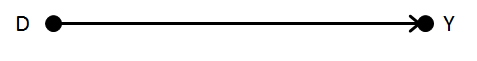
\includegraphics[width=0.7\textwidth]{Graphics/D_on_Y.png}
  \end{figure}
  
  \begin{table}[]
    \begin{tabular}{cc}
    \hline \hline
    \textbf{D}           & \textbf{Y}         \\ \hline
    Treatment variable   & Outcome variable   \\
    Explanatory variable  & Explained variable  \\
    Independent variable & Dependent variable \\ \hline \hline
    \end{tabular}
  \end{table}
  
\end{frame}


\begin{frame}{Criteria for causal inference (D on Y)}
  \begin{enumerate} 
    \item \textbf{Distinct theoretical constructs}: No definitional dependency between D and Y
    \item \textbf{Appropriate operationalizations and measurement} of both features: features $\rightarrow$ variables
    \item \textbf{Theoretical plausibility}: Qualitative explanation ($\rightarrow$ mechanism) of the causal effect necessary; reference to empirical studies not sufficient!
    \item \textbf{Appropriate temporal \underline{order}}: Theoretical justification needed (empirical order not sufficient, since anticipation effects can occur)
    \item \textbf{Appropriate temporal \underline{distance}}: Some effects take time to unfold and some effects weaken over time (theoretical justification needed)
    \item \textbf{Identification of the causal effect}: E.g. by DAG
    \item \textbf{Empirical association}: E.g. by regression analysis
  \end{enumerate}
\end{frame}


\section{The counterfactual causal model} % Wichtig für Inhaltsverzeichnis


\begin{frame}{History and basic idea}
\textbf{History}
  \begin{itemize}
    \item First approaches: John Stuart Mill 1843 \& Gustav Theodor Fechner 1860)
    \item Formal concepts of experimental designs in statistics: Neyman 1923 \& Fisher 1935
    \item Formalized causal analysis: Donald B. Rubin 1974, 1977 \& 1978
  \end{itemize}
\textbf{Basic idea}  
  \begin{itemize}
    \item Focus on the causality concept ''Estimating the causal effect of D on Y''
    \item Based on experimental language: almost any situation can be described in non-experimental context at least as a thought experiment
  \end{itemize}  
\textbf{Other names:}  
  \begin{itemize}
    \item Potential Outcome Model (POM)
    \item Rubin Causal Model (RCM)
    \item Modern Causal Analysis (MCA)
  \end{itemize}   
\end{frame}


\begin{frame}{Definitions of treatment and outcomes}
  \begin{figure}
	\centering
	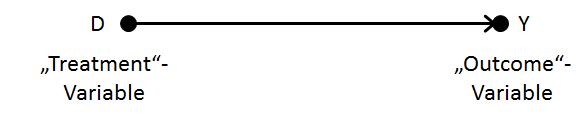
\includegraphics[width=0.7\textwidth]{Graphics/D_on_Y_names.png}
  \end{figure}
\textbf{Simplified version of a binary “Treatment”:}
  \begin{itemize}
    \item D=1:	Treatment (''Experimental group'')
    \item D=0: No Treatment (''Control group'')
  \end{itemize}
\textit{Note: The binary treatment assumption is a simplistic assumption; There are counterfactual causal models with polytomic treatments (nominal, ordinal, metric).}
\end{frame}


\begin{frame}{Central assumption for outcome Y}
  \begin{figure}
	\centering
	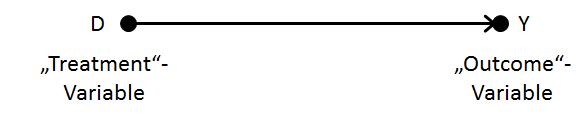
\includegraphics[width=0.7\textwidth]{Graphics/D_on_Y_names.png}
  \end{figure}
Each individual \textbf{i} can be observed in two potential states (depending on a potential treatment), which means that \textbf{two potential outcomes} are conceivable for each person \textbf{i}, regardless of the actual treatment status:
  \begin{itemize}
    \item Y\textsubscript{i}\textsuperscript{0} = potential outcome for person i in the case \underline{without} the treatment
    \item Y\textsubscript{i}\textsuperscript{1} = potential outcome for person i in the case of the treatment
  \end{itemize}
\textit{Note: The outcome is generally viewed as metric, but other scale levels can also be assumed.}
\end{frame}


\begin{frame}{Fundamental problem of causal inference}
\textbf{Fundamental problem of causal inference (Paul W. Holland, 1986):} \\
Y\textsubscript{i}\textsuperscript{0} and Y\textsubscript{i}\textsuperscript{1} can never be observed simultaneously for a \textit{single person i}

\begin{table}[]
\caption{Observability of various potential outcomes}
\begin{tabular}{ccc}
\hline \hline
\textbf{}                     & \textbf{Y\textsubscript{i}\textsuperscript{0}}                                                   & \textbf{Y\textsubscript{i}\textsuperscript{1}}                                                   \\ \hline
\textbf{D\textsubscript{i}=0} & {\color[HTML]{009901} \begin{tabular}[c]{@{}c@{}}Factual  \\ (=observable)\end{tabular}}       & {\color[HTML]{9A0000} \begin{tabular}[c]{@{}c@{}}Counterfactual\\ (=unobservable)\end{tabular}} \\
\textbf{D\textsubscript{i}=1} & {\color[HTML]{9A0000} \begin{tabular}[c]{@{}c@{}}Counterfactual\\ (=unobservable)\end{tabular}} & {\color[HTML]{009901} \begin{tabular}[c]{@{}c@{}}Factual \\ (=observable)\end{tabular}}        \\ \hline \hline
\end{tabular}
\end{table}

\textit{Observation rule: Given the actual state (D), only one potential outcome (Y) can be observed per person}
\end{frame}



\begin{frame}{Example of the problem}
\begin{scriptsize}
\begin{table}[]
\caption{Effect of (high) education on income}
\begin{tabular}{ccc}
\hline \hline
\textbf{}                     & \textbf{Y\textsubscript{i}\textsuperscript{0}}                                                                                                                  & \textbf{Y\textsubscript{i}\textsuperscript{1}}                                                                                                                  \\ \hline
\textbf{D\textsubscript{i}=0} & {\color[HTML]{009901} \begin{tabular}[c]{@{}c@{}}(''What a low-educated person \\ actually earns in \\ a state of low-education'')\end{tabular}}            & {\color[HTML]{9A0000} \begin{tabular}[c]{@{}c@{}}(''What a low-educated person \\ would earn if higher \\ education had been achieved'')\end{tabular}} \\
\textbf{D\textsubscript{i}=1} & {\color[HTML]{9A0000} \begin{tabular}[c]{@{}c@{}}(''What a high-educated person \\ would earn if low \\ education had been achieved'')\end{tabular}} & {\color[HTML]{009901} \begin{tabular}[c]{@{}c@{}}(''What a high-educated person \\ actually earns in \\ a state of high-education'')\end{tabular}}                   \\ \hline \hline
\end{tabular}
\end{table}
\end{scriptsize}
\textbf{Interpretation} (first line): If the person is actually low-educated ($\rightarrow$ no treatment), their income can be observed as if that person were low-educated. But \textit{\textbf{it can never be observed what income this person would have with a higher education}}.
\end{frame}


\begin{frame}{Impossibility of individual causal effects}
The \textit{individual causal effect} of the treatment on the outcome is defined for each individual as the difference between the two potential outcomes in the treatment and control status (given its actual D):\\
\textbf{Individual causal effect of a person i} = Y\textsubscript{i,D}\textsuperscript{1} - Y\textsubscript{i,D}\textsuperscript{0} \\[1em]
\textit{Implications:} 
  \begin{itemize}
    \item Theoretically the individual causal effect is defined
    \item In reality the individual causal effect can never be observed, because always one of the both components (Y\textsubscript{i}\textsuperscript{1} or Y\textsubscript{i}\textsuperscript{0}) is \textbf{contra factual} ($\rightarrow$ red in the table) and therefore unobservable
  \end{itemize}
\end{frame}


\begin{frame}{Solution: Average causal effects}
As social scientists, we are more interested in \textit{average causal effects} and not in the individual causal effect:

\textbf{Types of average effects:}
  \begin{itemize}
    \item \textit{ATT: Average Treatment Effect on the Treated}
    \item \textit{ATU: Average Treatment Effect on the Untreated}
    \item \textit{ATE: Average Treatment Effect}
  \end{itemize}

\end{frame}

\begin{frame}{Advanced notion of potential outcomes}
\begin{table}[]
\caption{Observability of various potential outcomes}
\begin{tabular}{ccc}
\hline \hline
\textbf{}                     & \textbf{Y\textsuperscript{0}}                                                   & \textbf{Y\textsuperscript{1}}                                                   \\ \hline
\textbf{D\textsubscript{i}=0} & {\color[HTML]{009901} \begin{tabular}[c]{@{}c@{}}E(Y\textsuperscript{0}$\vert$D=0) \\ Factual  \\ (=observable)\end{tabular}}       & {\color[HTML]{9A0000} \begin{tabular}[c]{@{}c@{}}E(Y\textsuperscript{1}$\vert$D=0) \\ Counterfactual\\ (=unobservable)\end{tabular}} \\
\textbf{D\textsubscript{i}=1} & {\color[HTML]{9A0000} \begin{tabular}[c]{@{}c@{}}E(Y\textsuperscript{0}$\vert$D=1) \\ Counterfactual\\ (=unobservable)\end{tabular}} & {\color[HTML]{009901} \begin{tabular}[c]{@{}c@{}}E(Y\textsuperscript{1}$\vert$D=1) \\ Factual \\ (=observable)\end{tabular}}        \\ \hline \hline
\end{tabular}
\end{table}

\vspace{10mm}
\small E() denotes the expected value = \href{https://en.wikipedia.org/wiki/Expected_value}{a generalization of the weighted average}
\end{frame}

\begin{frame}{Description of the concepts: ATT}
The \textit{ATT} is the average causal effect of the treatment on the outcome for people who actually experienced the treatment.
\begin{figure}
\centering
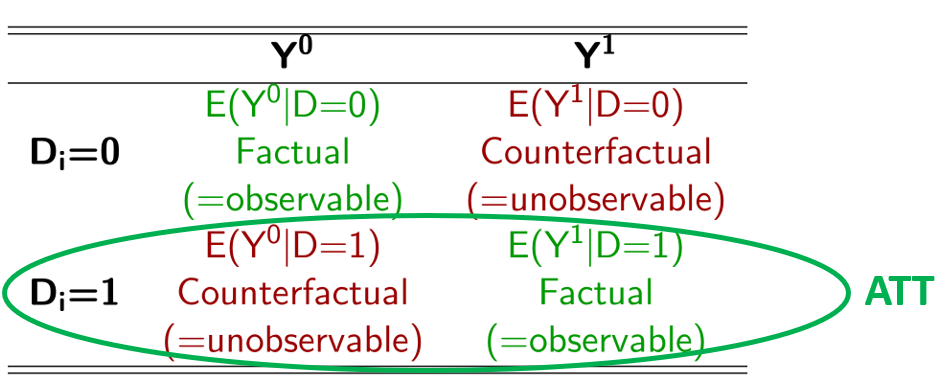
\includegraphics[width=1\textwidth]{Graphics/ATT.png}
\end{figure}
\begin{equation}
ATT = \underbrace{E(Y\textsubscript{i}\textsuperscript{1} \vert D\textsubscript{i}=1)}_\text{observable} - \underbrace{E(Y\textsubscript{i}\textsuperscript{0} \vert D\textsubscript{i}=1)}_\text{unobservable}
\end{equation} 

\small\textit{Research designs differ in how the unobservable/counterfactual situation is simulated / estimated.}
\end{frame}


\begin{frame}{Description of the concepts: ATU/ATNT}
The \textit{ATNT} is the average causal effect of the treatment on the outcome for people who didn't experienced the treatment.
\begin{figure}
\centering
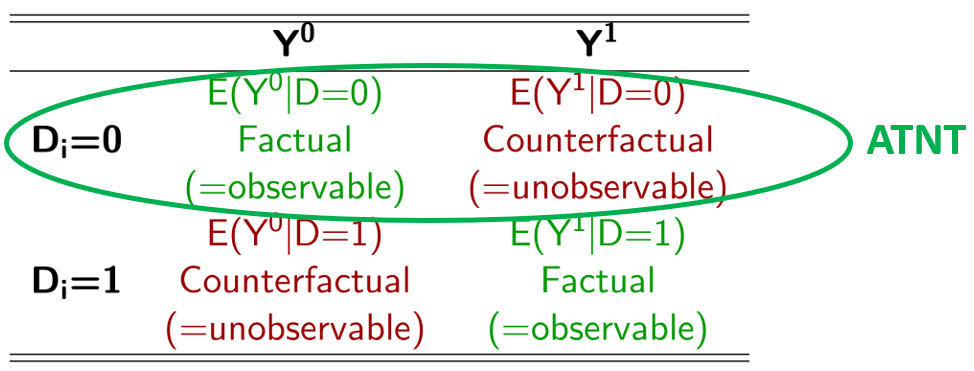
\includegraphics[width=1\textwidth]{Graphics/ATNT.png}
\end{figure}
\begin{equation}
ATNT = \underbrace{E(Y\textsubscript{i}\textsuperscript{1} \vert D\textsubscript{i}=0)}_\text{unobservable} - \underbrace{E(Y\textsubscript{i}\textsuperscript{0} \vert D\textsubscript{i}=0)}_\text{observable}
\end{equation} 

\small\textit{Research designs differ in how the unobservable/counterfactual situation is simulated / estimated.}
\end{frame}


\begin{frame}{Description of the concepts: ATE}
The \textit{ATE} is the average causal effect of the treatment on the outcome for all persons.
\begin{figure}
\centering
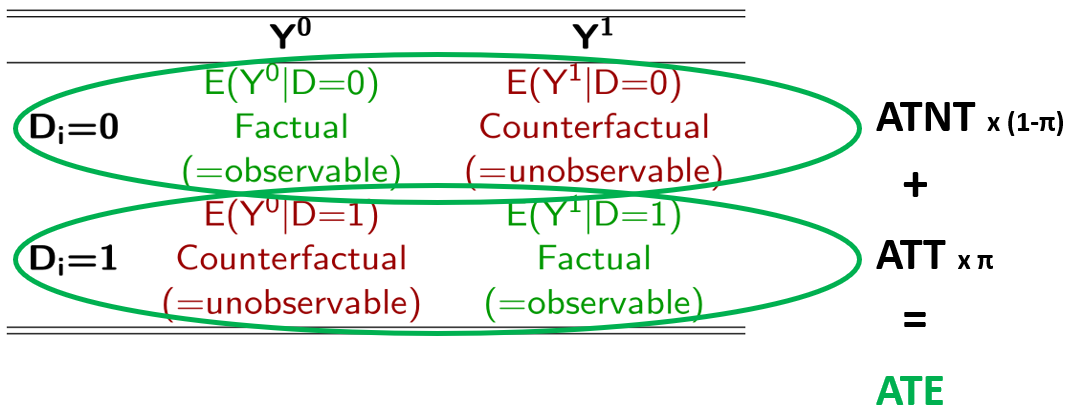
\includegraphics[width=1\textwidth]{Graphics/ATE.png}
\end{figure}
\begin{align*}
ATE &= \pi \times ATT + (1-\pi) \times ATNT \\
&= \pi \times (\underbrace{E(Y\textsubscript{i}\textsuperscript{1} \vert D\textsubscript{i}=1)}_\text{observable} - \underbrace{E(Y\textsubscript{i}\textsuperscript{0} \vert D\textsubscript{i}=1)}_\text{unobservable}) \\
&+ (1-\pi) \times \underbrace{E(Y\textsubscript{i}\textsuperscript{1} \vert D\textsubscript{i}=0)}_\text{unobservable} - \underbrace{E(Y\textsubscript{i}\textsuperscript{0} \vert D\textsubscript{i}=0)}_\text{observable}
\end{align*}
\end{frame}



\begin{frame}{Example}
\textit{The causal effect of higher education on income} \\[2em]
  \begin{itemize}
    \item \textbf{ATT} = Average causal effect of higher education on income for more high-educated people
    \item \textbf{ATNT} = Average causal effect of higher education on income for low-educated people
   \item \textbf{ATE} = Average causal effect of higher education on income \textit{(across all groups)}
  \end{itemize}
\end{frame}


\section{The naive estimator} % Wichtig für Inhaltsverzeichnis

\begin{frame}{Measurement problem: Counterfactual states}
Data is required for the empirical calculation of the effects. However, because some potential outcomes are counterfactual, it is not possible to calculate any of the average causal effects directly. \\
\textit{Nevertheless, we can only work with the existing data}

\begin{figure}
\centering
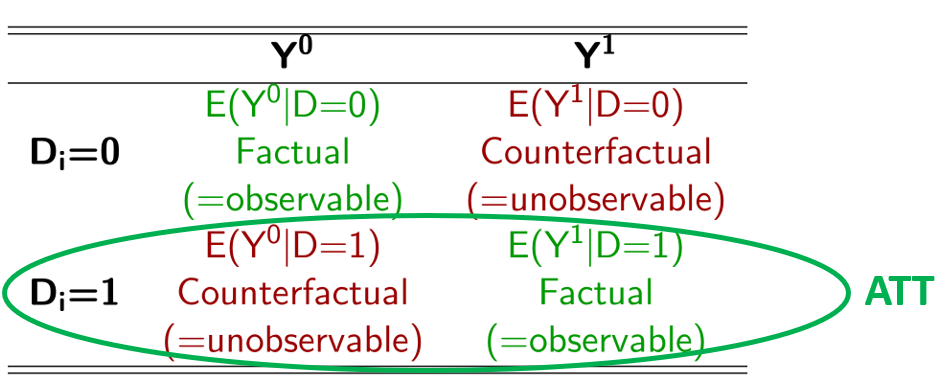
\includegraphics[width=0.5\textwidth]{Graphics/ATT.png}
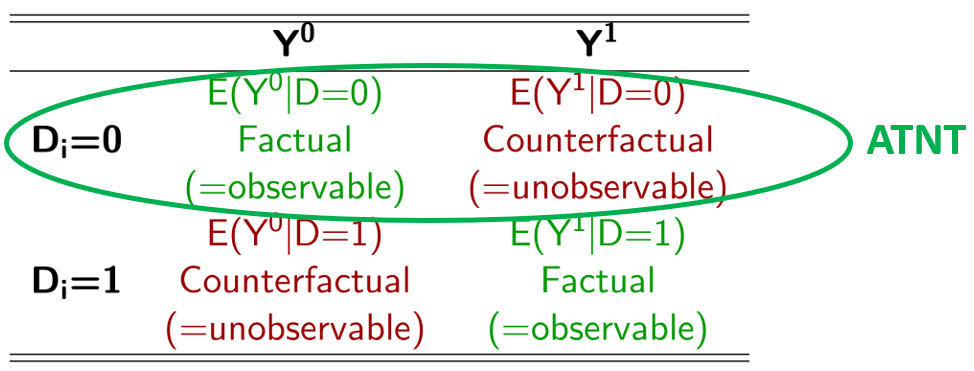
\includegraphics[width=0.5\textwidth]{Graphics/ATNT.png}
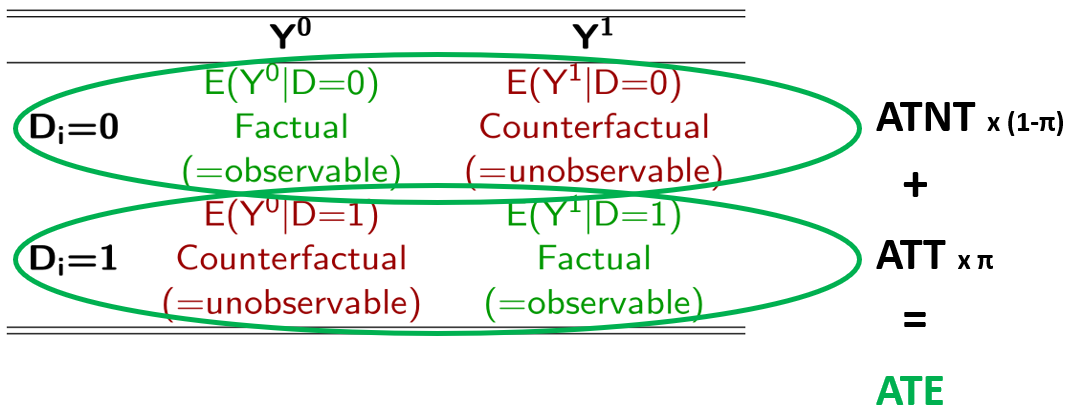
\includegraphics[width=0.5\textwidth]{Graphics/ATE.png}
\end{figure}
\end{frame}


\begin{frame}{Limited solution: The naive estimator}
\textbf{Definition}\\
The \textit{naive estimator (NaivE)} is the difference between the factual (observable) outcomes
\begin{align*}
NaivE = \underbrace{E(Y\textsubscript{i}\textsuperscript{1} \vert D\textsubscript{i}=1)}_\text{observable} - \underbrace{E(Y\textsubscript{i}\textsuperscript{0} \vert D\textsubscript{i}=0)}_\text{observable}
\end{align*}
\begin{figure}
\centering
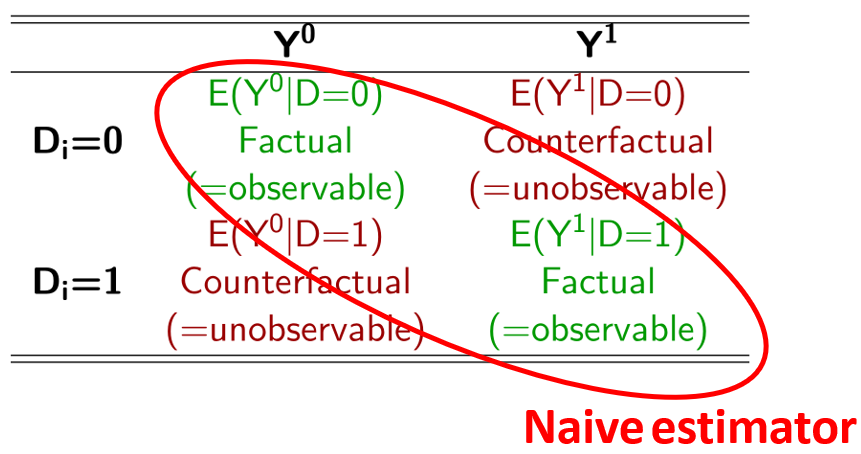
\includegraphics[width=1\textwidth]{Graphics/Naive.png}
\end{figure}
\end{frame}


\begin{frame}{The naive estimator: Example}
\begin{table}[]
\caption{Effect of high education on income}
\begin{tabular}{ccc}
\hline
\textbf{}                     & \textbf{Y\textsubscript{i}\textsuperscript{0}} & \textbf{Y\textsubscript{i}\textsuperscript{1}} \\ \hline
\textbf{D\textsubscript{i}=0} & {\color[HTML]{000000} 10 \euro/h}                  & {\color[HTML]{000000} 20 \euro/h}                   \\
\textbf{D\textsubscript{i}=1} & {\color[HTML]{000000} 15 \euro/h}                  & {\color[HTML]{000000} 30 \euro/h}                  \\ \hline
\end{tabular}
\end{table}
Calculation of the effect of high education on income:\\
\begin{itemize}
  \item \textcolor{red}{Naive estimator = 30 \euro/h - 10 \euro/h = \textbf{20 \euro/h}}
  \item ATT = 30 \euro/h - 15 \euro/h = \textcolor{green}{\textbf{15 \euro/h}}
  \item ATNT = 20 \euro/h - 10 \euro/h = \textcolor{green}{\textbf{10 \euro/h}}
  \item ATE = 15 \euro/h$\times \pi$ + 10 \euro/h $\times (1-\pi)$ = \textcolor{green}{\textbf{12.5 \euro/h}}
\end{itemize}
\end{frame}


\begin{frame}{Bias of the naive estimator}
\begin{itemize}
  \item In most of the real world scenarios, the naive estimator does not provide the true value of any causal effect. This means the result of the Naive Estimator is \textit{biased}! 
  \item This distortion results from the so-called \textbf{baseline difference}. This is the difference between the technically required but counterfactual potential outcome and the observable potential outcome used
\end{itemize}
\begin{figure}
\centering
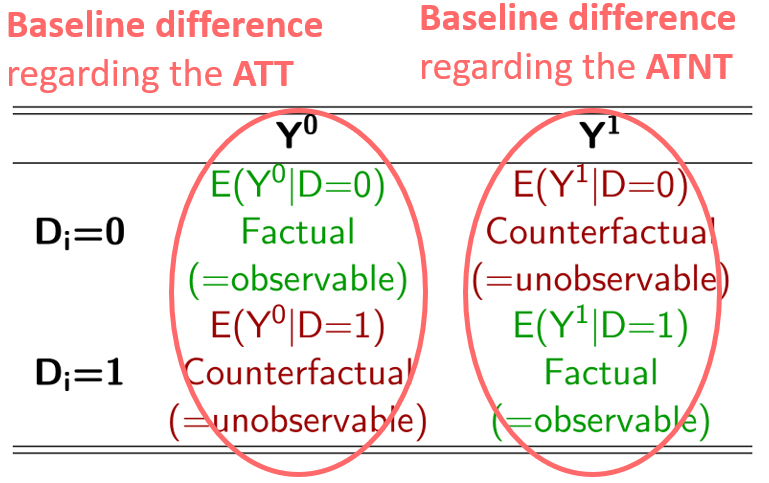
\includegraphics[width=0.7\textwidth]{Graphics/BaselineDifferences.png}
\end{figure}
\end{frame}


\begin{frame}{Bias decomposition: NaivE-ATT I}
\textit{Bias decomposition of the naive estimator (regarding ATT):}
\begin{align*}
NaivE &= E(Y\textsubscript{i}\textsuperscript{1}\vert D\textsubscript{i}=1)-E(Y\textsubscript{i}\textsuperscript{0} \vert D\textsubscript{i}=0) \\
&= ATT + \underbrace{(\underbrace{E(Y\textsubscript{i}\textsuperscript{0} \vert D\textsubscript{i}=1)}_\text{unobservable} - E(Y\textsubscript{i}\textsuperscript{0} \vert D\textsubscript{i}=0)}_\text{baseline difference})
\end{align*}
\begin{figure}
\centering
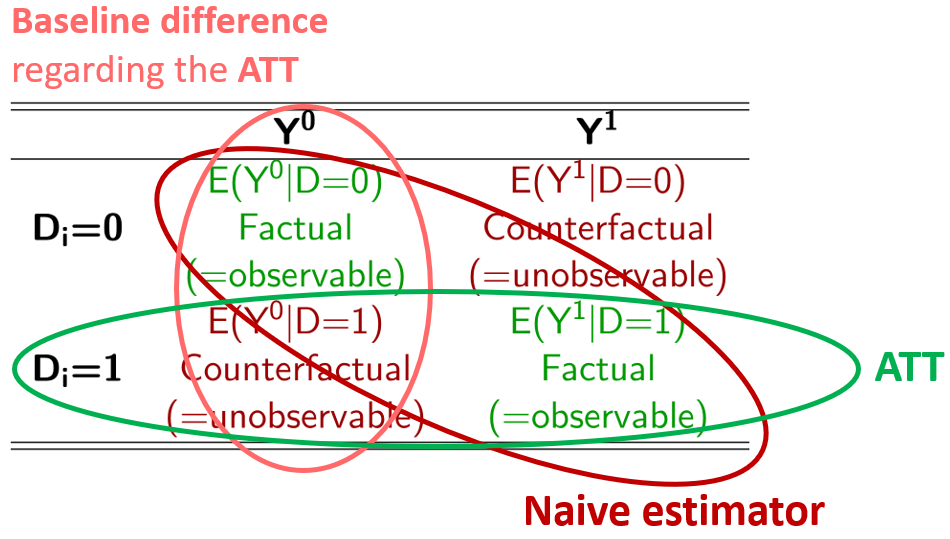
\includegraphics[width=0.8\textwidth]{Graphics/Naive_ATT_Baseline.png}
\end{figure}
\end{frame}

\begin{frame}{Bias decomposition: NaivE-ATT II}
\textbf{Calculation of the ATT from the naive estimator and the baseline difference.}
\\[1em]
Changing the formula of NaivE to ATT: \\
\begin{align*}
ATT = NaivE - \underbrace{(\underbrace{E(Y\textsubscript{i}\textsuperscript{0} \vert D\textsubscript{i}=1)}_\text{unobservable}- E(Y\textsubscript{i}\textsuperscript{0} \vert D\textsubscript{i}=0))}_\text{baseline difference}
\end{align*}
\\[1em]
Application:\\
In the example the baseline difference is (15 Euro/h - 10 Euro/h =) \textbf{5 Euro/h}. Naive estimator minus blaseline difference (20 Euro/h - 5 Euro/h) equals the true value of the ATT (15 Euro/h)
\end{frame}



\begin{frame}{Bias decomposition: NaivE-ATNT I}
\textit{Bias decomposition of the naive estimator (regarding ATNT):}
\begin{align*}
NaivE &= E(Y\textsubscript{i}\textsuperscript{1}\vert D\textsubscript{i}=1)-E(Y\textsubscript{i}\textsuperscript{0} \vert D\textsubscript{i}=0) \\
&= ATNT + (\underbrace{E(Y\textsubscript{i}\textsuperscript{1} \vert D\textsubscript{i}=1) - \underbrace{E(Y\textsubscript{i}\textsuperscript{1} \vert D\textsubscript{i}=0)}_\text{unobservable})}_\text{baseline difference}
\end{align*}
\begin{figure}
\centering
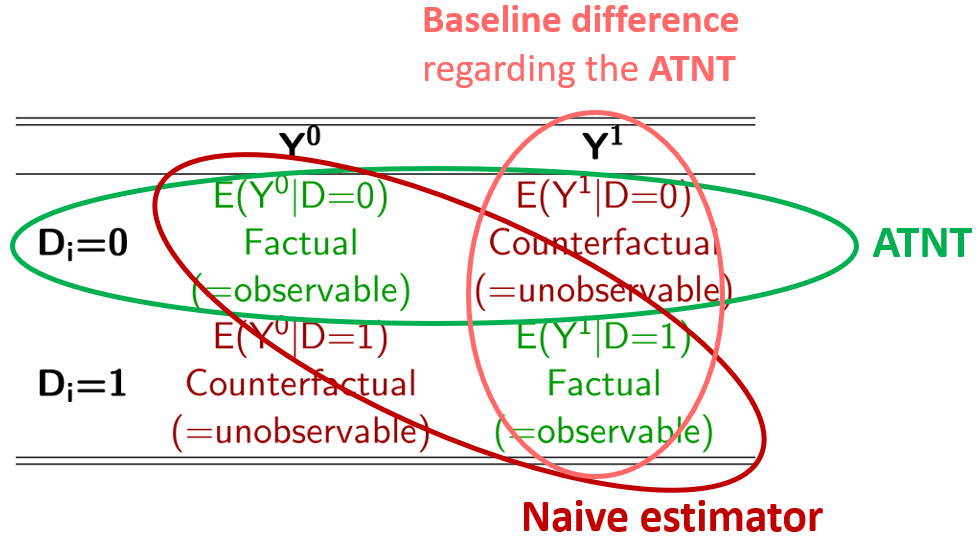
\includegraphics[width=0.8\textwidth]{Graphics/Naive_ATNT_Baseline.png}
\end{figure}
\end{frame}

\begin{frame}{Bias decomposition: NaivE-ATNT II}
\textbf{Calculation of the ATT from the naive estimator and the baseline difference.}
\\[1em]
Changing the formula of NaivE to ATNT: \\
\begin{align*}
ATNT = NaivE - \underbrace{(E(Y\textsubscript{i}\textsuperscript{1} \vert D\textsubscript{i}=1) - \underbrace{E(Y\textsubscript{i}\textsuperscript{1} \vert D\textsubscript{i}=0)}_\text{unobservable})}_\text{baseline difference}
\end{align*}
\\[1em]
Application:\\
In the example the baseline difference is (30 Euro/h - 20 Euro/h =) \textbf{10 Euro/h}. Naive estimator minus blaseline difference (20 Euro/h - 10 Euro/h) equals the true value of the ATNT (10 Euro/h)
\end{frame}


\begin{frame}{Violation of the ignorability assumption}
\textbf{Reason for the bias of the naive estimator} 
\\
$\rightarrow$ Violation of the \textit{Ignorability Assumption (IA)} 
\\[1em]
\textbf{IA:} (Y\textsuperscript{0},Y\textsuperscript{1}) $\upmodels$ D 
\\
$\Rightarrow$ E(Y\textsuperscript{0}$\vert$D=0) = E(Y\textsuperscript{0}$\vert$D=1) = E(Y\textsuperscript{0}) 
\\
$\Rightarrow$ E(Y\textsuperscript{1}$\vert$D=0) = E(Y\textsuperscript{1}$\vert$D=1) = E(Y\textsuperscript{1})

\begin{itemize}
\item Assignment of the treatment status D is independent of the potential outcome
\item Caution: The ignorability assumption is often not fulfilled (due to a lack of randomization), since features in the background influence both individuals assignment of the treatment group and their potential outcomes $\rightarrow$ distortion of the naive estimator
\end{itemize}
\end{frame}


\begin{frame}{Ignorability assumption}
\textbf{Implication of the ignorability assumption}
\\[1em]
\begin{itemize}
  \item If it applies, the potential outcomes are independent of treatment status D.\\
\end{itemize}
Thus applies:
\\
E(Y\textsuperscript{0}$\vert$D=1) = E(Y\textsuperscript{0}$\vert$D=0) and 
\\
E(Y\textsuperscript{1}$\vert$D=1) = E(Y\textsuperscript{1}$\vert$D=0)
\\[1em]
\begin{itemize}
\item From this, in turn, it follows that the baseline difference (the bias of NaiveS) is: (E[Y\textsubscript{i}\textsuperscript{0}$\vert$D\textsubscript{i}=1] - E[Y\textsubscript{i}\textsuperscript{0}$\vert$D\textsubscript{i}=0] =) 0 
\item \textit{The NaiveS thus results in the true average causal effect of interest (ATT,ATNT or ATE)}
\end{itemize}

\end{frame}


\begin{frame}{Ignorability assumption}
\textbf{Under which conditions is the ignorability assumption valid?}
\begin{enumerate}
  \item Treatment status D is in fact independent of the potential outcomes
  \item Treatment status D is after conditioning a set of variables Z independent of the potential outcomes $\rightarrow$ \textit{Conditional Ignorability Assumption (CIA)}
\end{enumerate}

\textbf{How can these conditions be verified?}
\begin{enumerate}
  \item With \textit{Directed Acyclic Graphs (DAGs)} (1) and (2) can be checked
  \item For (2), the required set of variables Z can be derived using DAGs
\end{enumerate}

\end{frame}


\section{Directed Acyclic Graphs (DAGs)} % Wichtig für Inhaltsverzeichnis

\begin{frame}{Directed Acyclic Graphs (DAGs)}
\textbf{Pearl 1995: Causal diagrams for empirical research}
\begin{itemize}
  \item Graphical tool to represent qualitative assumptions about causal relationships 
  \item It is possible to derive causal conclusions from these assumptions and data
\end{itemize}

\textbf{Notation}
\begin{itemize}
  \item Each point of the DAG represents a features/variable whose name is given
  \item Filled points represent \textit{observed} features/variables
  \item Unfilled points represent \textit{unobserved} features/variables
  \item One-sided arrows postulate a directed causal effect \textit{(theoretically or based on empirical causal analysis)}
\end{itemize}
\end{frame} 


\begin{frame}{Directed Acyclic Graphs (DAGs)}
\textbf{Definitions}
\begin{itemize}
  \item \textbf{Path:} Every (uninterrupted) connection between two points, \textit{regardless of the direction of the arrow}
  \item \textbf{Causal Path:} Every (uninterrupted) connection between two points, \textit{with clear arrow direction}
  \item \textbf{Directed Graph:} Every connection between two variables is a one-sided arrow
  \item \textbf{Acyclic Graph:} There are no loops of causal paths
  \item \textbf{Back-door Path:} A path that connects D and Y and in which an arrowhead points to D.
  \item \textbf{Collider:} A variable pointed to by two arrows
  \item \textbf{(Un-)Blocked Path:} A path is \textit {blocked} if there is at least one collider on it, otherwise this is \textit{unblocked}.
  \item \textbf{Blocking Paths:} A path can be blocked by a variable on this path that is not a collider
\end{itemize}
\end{frame} 


\begin{frame}{Directed Acyclic Graphs (DAGs)}
\textbf{Back-door criterion}
\\[1em]
A set of variables Z fulfills the \textit{back-door criterium} if:
\begin{itemize}
  \item No variable in Z is causally influenced by D.
  \item By Z every \textit{unblocked path} between D and Y becomes blocked
\end{itemize}
If the back-door criterion is met, the CIA is satisfied and a causal effect identified
\end{frame} 



%------------------------------------------------------%
%--------------------- DAG I --------------------------%
%------------------------------------------------------%

\begin{frame}{DAG Examples I: Overview}
\textbf{No Confounding}
\begin{figure}
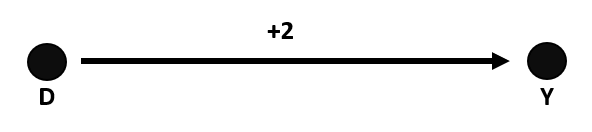
\includegraphics[width=0.8\textwidth]{{Graphics/1.NoConfounding.png}}
\end{figure}
Question:
\begin{enumerate}
\item What is the causal path of interest?
\item What is/are the back-door path(s)? Are they open? How to block them? \\[1em]
\end{enumerate}
$\rightarrow$ Is the result of the naive estimator the true causal effect?
\end{frame}

\begin{frame}{DAG Examples I: Paths}
\begin{figure}
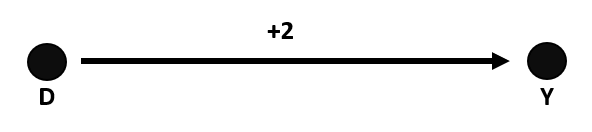
\includegraphics[width=0.8\textwidth]{{Graphics/1.NoConfounding.png}}
\end{figure}
\textbf{Paths:}
\begin{itemize}
\item Causal path: D $\rightarrow$ Y
\end{itemize}

\textbf{CIA satisfaction:}
\begin{itemize}
\item Automatically satisfied because there are no back-door path 
\end{itemize}
\end{frame}


\begin{frame}{DAG Examples I: Scatterplot}
\begin{figure}
\begin{knitrout}
\definecolor{shadecolor}{rgb}{0.969, 0.969, 0.969}\color{fgcolor}
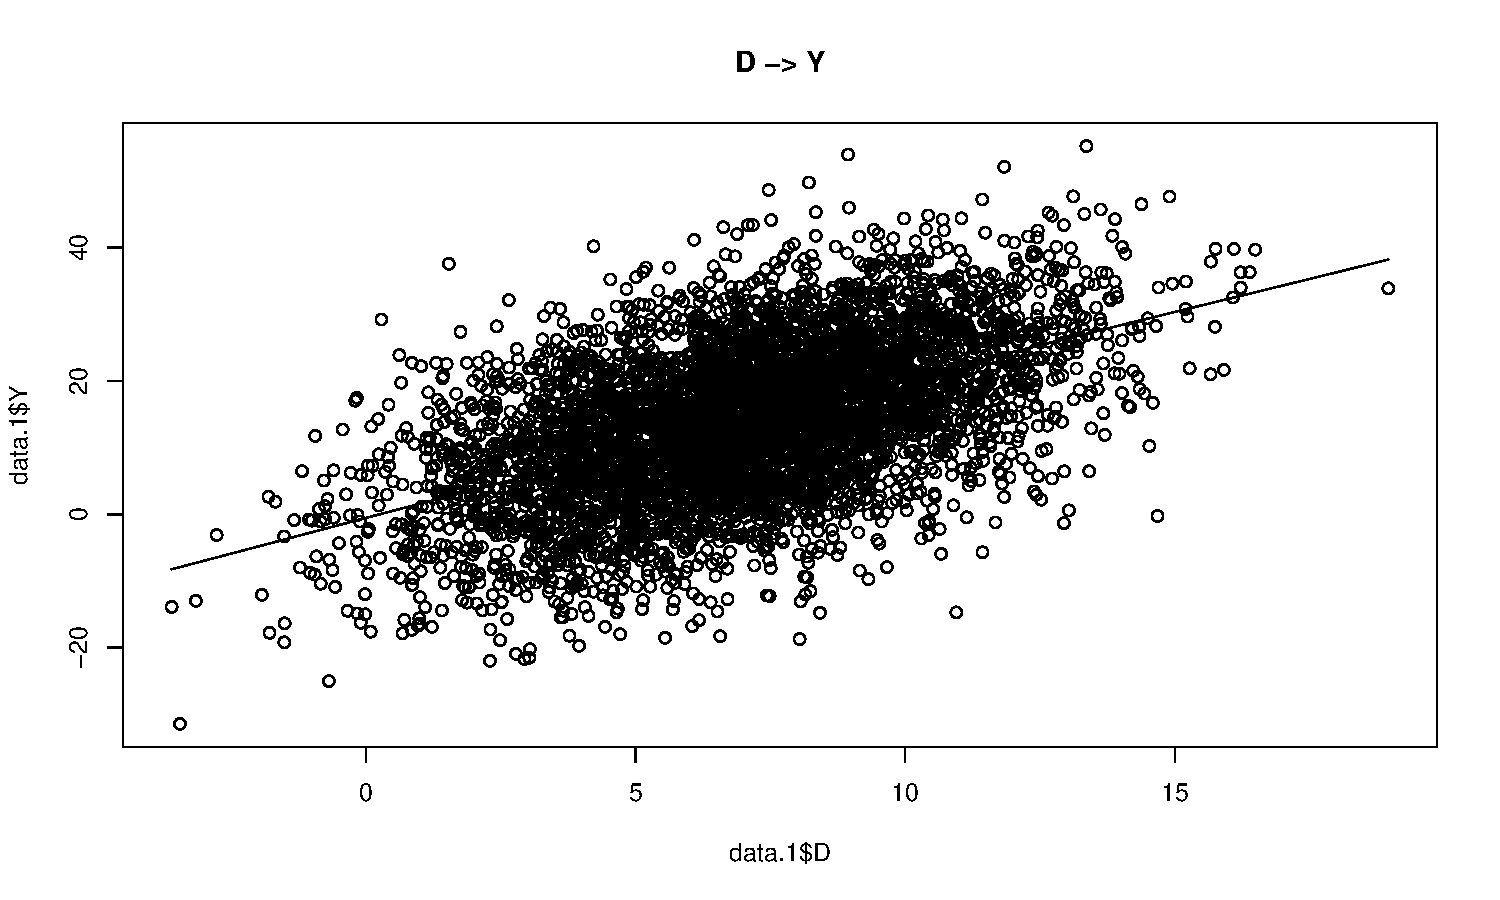
\includegraphics[width=\maxwidth]{figure/ExamplesIScatterplot-1} 
\end{knitrout}
\end{figure}
\end{frame}


\begin{frame}[fragile]{DAG Examples I: Regression result}
% latex table generated in R 4.2.1 by xtable 1.8-4 package
% Fri Dec 16 17:22:32 2022
\begin{table}[ht]
\centering
\begin{tabular}{rrrrr}
  \hline
 & Estimate & Std. Error & t value & Pr($>$$|$t$|$) \\ 
  \hline
(Intercept) & -0.4878 & 0.3583 & -1.36 & 0.1735 \\ 
  D & 2.0578 & 0.0472 & 43.58 & 0.0000 \\ 
   \hline
\end{tabular}
\caption{Regression: lm(Y \textasciitilde ~D)} 
\end{table}
% latex table generated in R 4.2.1 by xtable 1.8-4 package
% Fri Dec 16 17:22:32 2022
\begin{table}[ht]
\centering
\begin{tabular}{rrr}
  \hline
 & 2.5 \% & 97.5 \% \\ 
  \hline
D & 1.97 & 2.15 \\ 
   \hline
\end{tabular}
\caption{95-Percent confidence interval} 
\end{table}

\end{frame}



%------------------------------------------------------%
%--------------------- DAG II -------------------------%
%------------------------------------------------------%


\begin{frame}{DAG Examples II: (Partially) Covered}
\\[1em]
\begin{figure}
\includegraphics[width=0.6\textwidth]{Graphics/2.SimpleConfounding-Covered.png}
\end{figure}
Question:
\begin{enumerate}
\item What is the causal path of interest?
\item What is/are the back-door path(s)? Are they open? How to block them?
\end{enumerate}
\\[1em]
$\rightarrow$ Is the result of the naive estimator the true causal effect?
\end{frame}


\begin{frame}{DAG Examples II: Paths}
\begin{figure}
\includegraphics[width=0.8\textwidth]{{Graphics/2.SimpleConfounding-Covered.png}}
\end{figure}
\textbf{Paths:}
\begin{itemize}
\item Causal path: D $\rightarrow$ Y
\item Back-door path: D $\leftarrow$ C $\rightarrow$ Y
\end{itemize}

\textbf{CIA satisfaction:}
\begin{itemize}
\item Z1 = \{C\}
\end{itemize}
\end{frame}


\begin{frame}{DAG Examples II: Scatterplot}
\begin{figure}
\begin{knitrout}
\definecolor{shadecolor}{rgb}{0.969, 0.969, 0.969}\color{fgcolor}
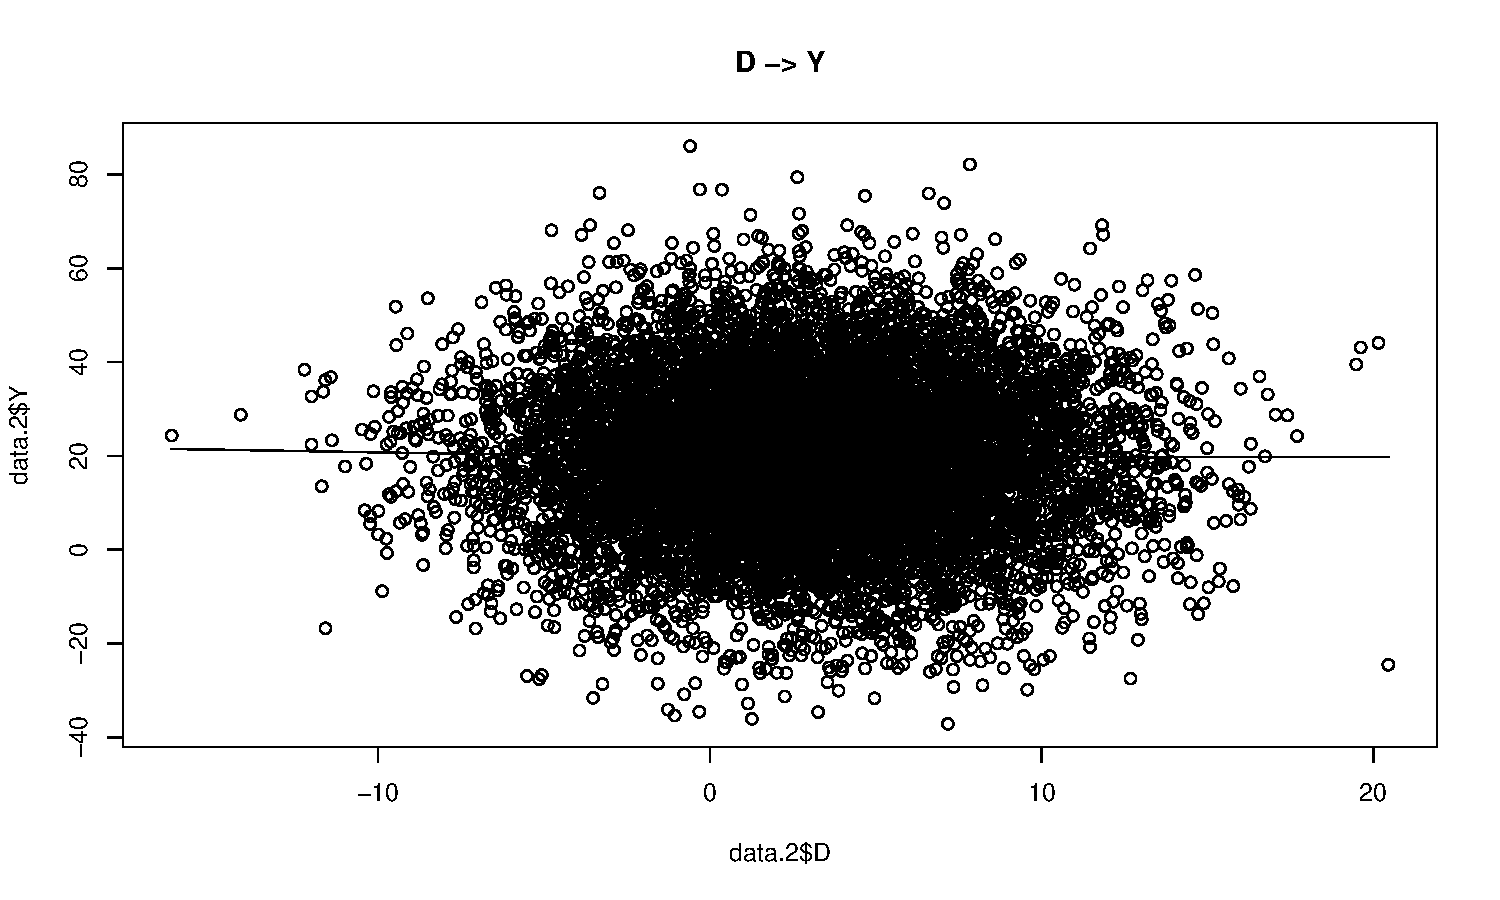
\includegraphics[width=\maxwidth]{figure/ExamplesIIScatterplot-1} 
\end{knitrout}
\end{figure}
\end{frame}


\begin{frame}[fragile]{DAG Examples II: Regression result, NaivE}
% latex table generated in R 4.2.1 by xtable 1.8-4 package
% Fri Dec 16 17:22:32 2022
\begin{table}[ht]
\centering
\begingroup\small
\begin{tabular}{rrrrr}
  \hline
 & Estimate & Std. Error & t value & Pr($>$$|$t$|$) \\ 
  \hline
(Intercept) & 19.9093 & 0.1995 & 99.80 & 0.0000 \\ 
  D & -0.0443 & 0.0366 & -1.21 & 0.2256 \\ 
   \hline
\end{tabular}
\endgroup
\caption{Regression: lm(Y \textasciitilde ~D)} 
\end{table}
% latex table generated in R 4.2.1 by xtable 1.8-4 package
% Fri Dec 16 17:22:32 2022
\begin{table}[ht]
\centering
\begingroup\small
\begin{tabular}{rrr}
  \hline
 & 2.5 \% & 97.5 \% \\ 
  \hline
D & -0.12 & 0.03 \\ 
   \hline
\end{tabular}
\endgroup
\caption{95-Percent confidence interval: lm(Y \textasciitilde ~D)} 
\end{table}

\end{frame}

\begin{frame}[fragile]{DAG Examples II: Regression result, CIA}
\textbf{Usage of Z1 to satisfy CIA}
% latex table generated in R 4.2.1 by xtable 1.8-4 package
% Fri Dec 16 17:22:32 2022
\begin{table}[ht]
\centering
\begingroup\small
\begin{tabular}{rrrrr}
  \hline
 & Estimate & Std. Error & t value & Pr($>$$|$t$|$) \\ 
  \hline
(Intercept) & -0.0086 & 0.4110 & -0.02 & 0.9834 \\ 
  D & 1.9542 & 0.0493 & 39.65 & 0.0000 \\ 
  C & 3.4925 & 0.0651 & 53.62 & 0.0000 \\ 
   \hline
\end{tabular}
\endgroup
\caption{Regression: lm(Y \textasciitilde ~D + C1)} 
\end{table}
% latex table generated in R 4.2.1 by xtable 1.8-4 package
% Fri Dec 16 17:22:32 2022
\begin{table}[ht]
\centering
\begingroup\small
\begin{tabular}{rrr}
  \hline
 & 2.5 \% & 97.5 \% \\ 
  \hline
D & 1.86 & 2.05 \\ 
   \hline
\end{tabular}
\endgroup
\caption{95-Percent confidence interval: lm(Y \textasciitilde ~D + C1)} 
\end{table}

\end{frame}

%------------------------------------------------------%
%--------------------- DAG III ------------------------%
%------------------------------------------------------%

\begin{frame}{DAG Examples III: Oversized}
\\[1em]
\begin{figure}
\includegraphics[width=0.6\textwidth]{Graphics/3.SimpleConfounding-Oversized.png}
\end{figure}
Question:
\begin{enumerate}
\item What is the causal path of interest?
\item What is/are the back-door path(s)? Are they open? How to block them?
\end{enumerate}
\\[1em]
$\rightarrow$ Is the result of the naive estimator the true causal effect?
\end{frame}


\begin{frame}{DAG Examples III: Paths}
\begin{figure}
\includegraphics[width=0.8\textwidth]{{Graphics/3.SimpleConfounding-Oversized.png}}
\end{figure}
\textbf{Paths:}
\begin{itemize}
\item Causal path: D $\rightarrow$ Y
\item Back-door path: D $\leftarrow$ C $\rightarrow$ Y
\end{itemize}

\textbf{CIA satisfaction:}
\begin{itemize}
\item Z1 = \{C\}
\end{itemize}
\end{frame}


\begin{frame}{DAG Examples III: Scatterplot}
\begin{figure}
\begin{knitrout}
\definecolor{shadecolor}{rgb}{0.969, 0.969, 0.969}\color{fgcolor}
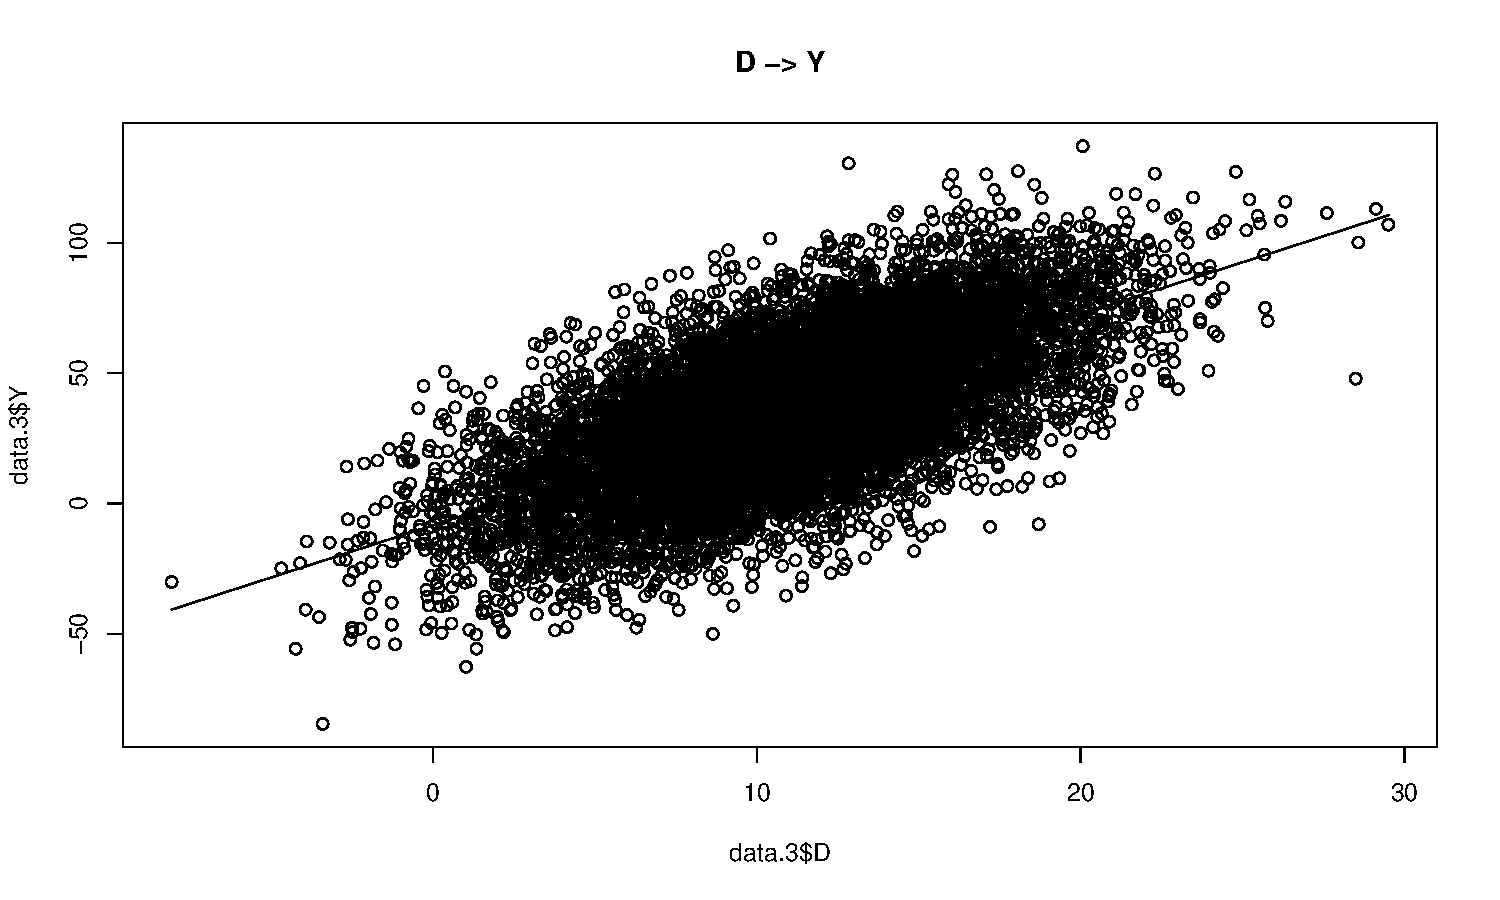
\includegraphics[width=\maxwidth]{figure/ExamplesIIIScatterplot-1} 
\end{knitrout}
\end{figure}
\end{frame}


\begin{frame}[fragile]{DAG Examples III: Regression result, NaivE}
% latex table generated in R 4.2.1 by xtable 1.8-4 package
% Fri Dec 16 17:22:32 2022
\begin{table}[ht]
\centering
\begingroup\small
\begin{tabular}{rrrrr}
  \hline
 & Estimate & Std. Error & t value & Pr($>$$|$t$|$) \\ 
  \hline
(Intercept) & -8.4145 & 0.5506 & -15.28 & 0.0000 \\ 
  D & 4.0103 & 0.0461 & 87.01 & 0.0000 \\ 
   \hline
\end{tabular}
\endgroup
\caption{Regression: lm(Y \textasciitilde ~D)} 
\end{table}
% latex table generated in R 4.2.1 by xtable 1.8-4 package
% Fri Dec 16 17:22:32 2022
\begin{table}[ht]
\centering
\begingroup\small
\begin{tabular}{rrr}
  \hline
 & 2.5 \% & 97.5 \% \\ 
  \hline
D & 3.92 & 4.10 \\ 
   \hline
\end{tabular}
\endgroup
\caption{95-Percent confidence interval: lm(Y \textasciitilde ~D)} 
\end{table}

\end{frame}

\begin{frame}[fragile]{DAG Examples III: Regression result, CIA}
\textbf{Usage of Z1 to satisfy CIA}
% latex table generated in R 4.2.1 by xtable 1.8-4 package
% Fri Dec 16 17:22:32 2022
\begin{table}[ht]
\centering
\begingroup\small
\begin{tabular}{rrrrr}
  \hline
 & Estimate & Std. Error & t value & Pr($>$$|$t$|$) \\ 
  \hline
(Intercept) & -0.3580 & 0.5460 & -0.66 & 0.5121 \\ 
  D & 1.9886 & 0.0652 & 30.51 & 0.0000 \\ 
  C & 3.5625 & 0.0868 & 41.02 & 0.0000 \\ 
   \hline
\end{tabular}
\endgroup
\caption{Regression: lm(Y \textasciitilde ~D + C1)} 
\end{table}
% latex table generated in R 4.2.1 by xtable 1.8-4 package
% Fri Dec 16 17:22:33 2022
\begin{table}[ht]
\centering
\begingroup\small
\begin{tabular}{rrr}
  \hline
 & 2.5 \% & 97.5 \% \\ 
  \hline
D & 1.86 & 2.12 \\ 
   \hline
\end{tabular}
\endgroup
\caption{95-Percent confidence interval: lm(Y \textasciitilde ~D + C1)} 
\end{table}

\end{frame}



%------------------------------------------------------%
%--------------------- DAG IV -------------------------%
%------------------------------------------------------%


\begin{frame}{DAG Examples IV}
\\[1em]
\begin{figure}
\centering
\includegraphics[width=0.6\textwidth]{Graphics/4.LongBack-doorPath-Oversized.png}
\end{figure}
Question:
\begin{enumerate}
\item What is the causal path of interest?
\item What is/are the back-door path(s)? Are they open? How to block them?
\end{enumerate}
\\[1em]
$\rightarrow$ Is the result of the naive estimator the true causal effect?
\end{frame}


\begin{frame}{DAG Examples IV: Paths}
\begin{figure}
\includegraphics[width=0.8\textwidth]{{Graphics/4.LongBack-doorPath-Oversized.png}}
\end{figure}
\textbf{Paths:}
\begin{itemize}
\item Causal path: D $\rightarrow$ Y
\item Back-door path: D $\leftarrow$ C\textsubscript{1} $\rightarrow$ C\textsubscript{2} $\rightarrow$ Y
\end{itemize}

\textbf{CIA satisfaction:}
\begin{itemize}
\item Z1 = \{C\textsubscript{1}\} or
\item Z2 = \{C\textsubscript{2}\}
\end{itemize}
\end{frame}


\begin{frame}{DAG Examples IV: Scatterplot}
\begin{figure}
\begin{knitrout}
\definecolor{shadecolor}{rgb}{0.969, 0.969, 0.969}\color{fgcolor}
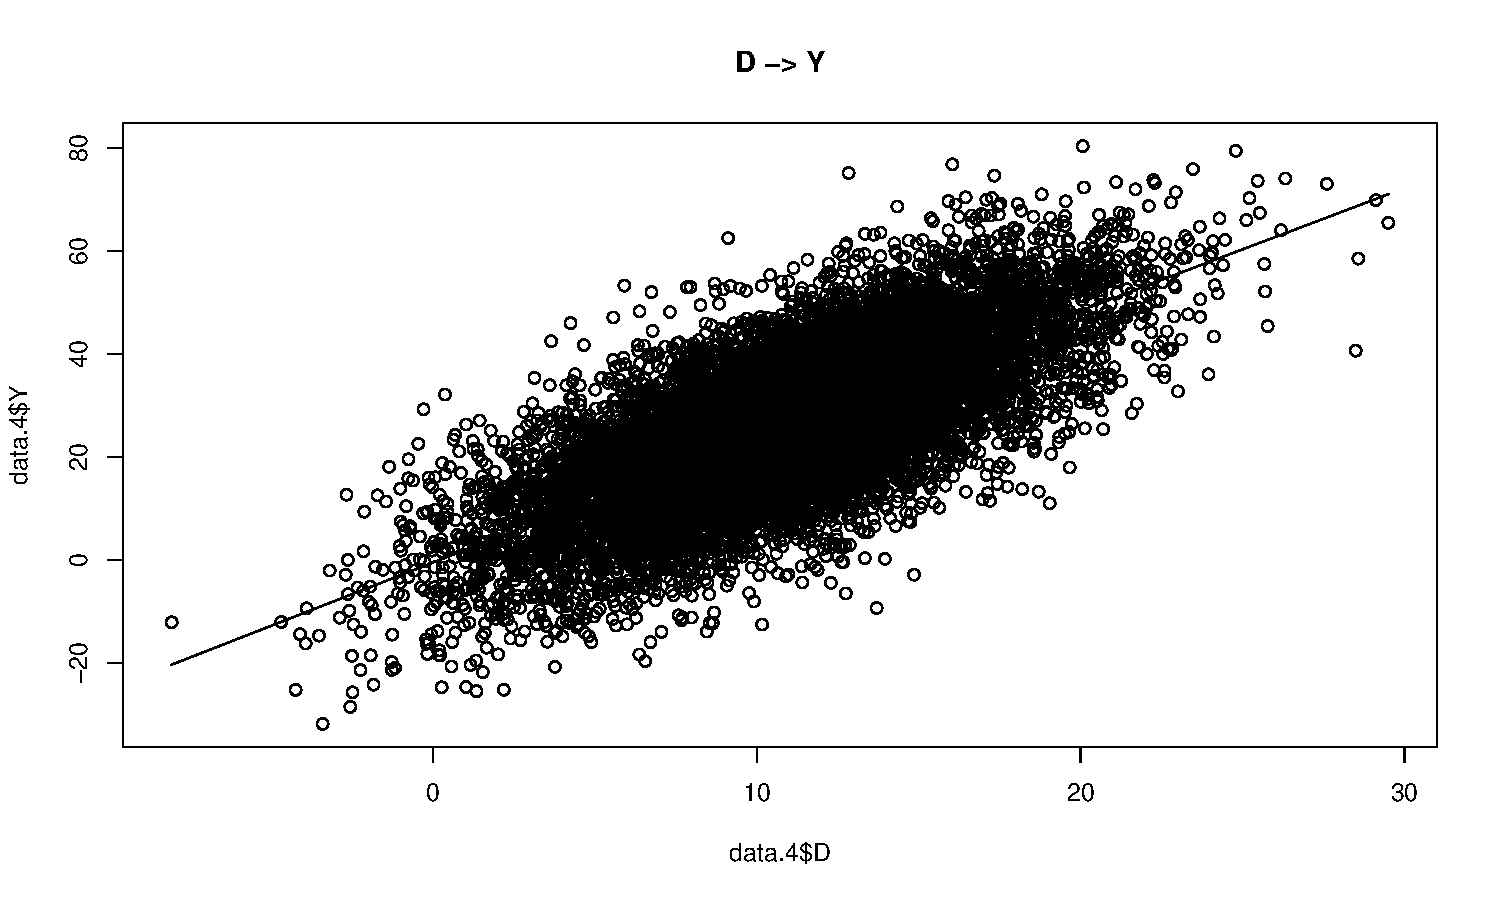
\includegraphics[width=\maxwidth]{figure/ExamplesIVScatterplot-1} 
\end{knitrout}
\end{figure}
\end{frame}


\begin{frame}[fragile]{DAG Examples IV: Regression result, NaivE}
% latex table generated in R 4.2.1 by xtable 1.8-4 package
% Fri Dec 16 17:22:33 2022
\begin{table}[ht]
\centering
\begingroup\small
\begin{tabular}{rrrrr}
  \hline
 & Estimate & Std. Error & t value & Pr($>$$|$t$|$) \\ 
  \hline
(Intercept) & -0.2863 & 0.2769 & -1.03 & 0.3011 \\ 
  D & 2.4241 & 0.0232 & 104.57 & 0.0000 \\ 
   \hline
\end{tabular}
\endgroup
\caption{Regression: lm(Y \textasciitilde ~D)} 
\end{table}
% latex table generated in R 4.2.1 by xtable 1.8-4 package
% Fri Dec 16 17:22:33 2022
\begin{table}[ht]
\centering
\begingroup\small
\begin{tabular}{rrr}
  \hline
 & 2.5 \% & 97.5 \% \\ 
  \hline
D & 2.38 & 2.47 \\ 
   \hline
\end{tabular}
\endgroup
\caption{95-Percent confidence interval: lm(Y \textasciitilde ~D)} 
\end{table}

\end{frame}

\begin{frame}[fragile]{DAG Examples IV: Regression result, CIA I}
\textbf{Usage of Z1 to satisfy CIA}
% latex table generated in R 4.2.1 by xtable 1.8-4 package
% Fri Dec 16 17:22:33 2022
\begin{table}[ht]
\centering
\begingroup\small
\begin{tabular}{rrrrr}
  \hline
 & Estimate & Std. Error & t value & Pr($>$$|$t$|$) \\ 
  \hline
(Intercept) & 1.5029 & 0.2926 & 5.14 & 0.0000 \\ 
  D & 1.9751 & 0.0349 & 56.54 & 0.0000 \\ 
  C1 & 0.7912 & 0.0465 & 17.00 & 0.0000 \\ 
   \hline
\end{tabular}
\endgroup
\caption{Regression: lm(Y \textasciitilde ~D + C1)} 
\end{table}
% latex table generated in R 4.2.1 by xtable 1.8-4 package
% Fri Dec 16 17:22:33 2022
\begin{table}[ht]
\centering
\begingroup\small
\begin{tabular}{rrr}
  \hline
 & 2.5 \% & 97.5 \% \\ 
  \hline
D & 1.91 & 2.04 \\ 
   \hline
\end{tabular}
\endgroup
\caption{95-Percent confidence interval: lm(Y \textasciitilde ~D + C1)} 
\end{table}

\end{frame}

\begin{frame}[fragile]{DAG Examples IV: Regression result, CIA II}
\textbf{Usage of Z2 to satisfy CIA}
% latex table generated in R 4.2.1 by xtable 1.8-4 package
% Fri Dec 16 17:22:33 2022
\begin{table}[ht]
\centering
\begingroup\small
\begin{tabular}{rrrrr}
  \hline
 & Estimate & Std. Error & t value & Pr($>$$|$t$|$) \\ 
  \hline
(Intercept) & -0.2489 & 0.2547 & -0.98 & 0.3285 \\ 
  D & 2.0035 & 0.0235 & 85.29 & 0.0000 \\ 
  C2 & 1.5313 & 0.0359 & 42.68 & 0.0000 \\ 
   \hline
\end{tabular}
\endgroup
\caption{Regression: lm(Y \textasciitilde ~D + C2)} 
\end{table}
% latex table generated in R 4.2.1 by xtable 1.8-4 package
% Fri Dec 16 17:22:33 2022
\begin{table}[ht]
\centering
\begingroup\small
\begin{tabular}{rrr}
  \hline
 & 2.5 \% & 97.5 \% \\ 
  \hline
D & 1.96 & 2.05 \\ 
   \hline
\end{tabular}
\endgroup
\caption{95-Percent confidence interval: lm(Y \textasciitilde ~D + C2)} 
\end{table}

\end{frame}

%------------------------------------------------------%
%--------------------- DAG V --------------------------%
%------------------------------------------------------%

\begin{frame}{DAG Examples V: (Partially) Covered}
\\[1em]
\begin{figure}
\centering
\includegraphics[width=0.6\textwidth]{Graphics/5.TwoBack-doorpaths-Covered.png}
\end{figure}
Question:
\begin{enumerate}
\item What is the causal path of interest?
\item What is/are the back-door path(s)? Are they open? How to block them?
\end{enumerate}
\\[1em]
$\rightarrow$ Is the result of the naive estimator the true causal effect?
\end{frame}


\begin{frame}{DAG Examples V: Paths}
\begin{figure}
\includegraphics[width=0.5\textwidth]{{Graphics/5.TwoBack-doorpaths-Covered.png}}
\end{figure}
\textbf{Paths:}
\begin{itemize}
\item Causal path: D $\rightarrow$ Y
\item 1. Back-door path: D $\leftarrow$ C\textsubscript{1} $\rightarrow$ C\textsubscript{2} $\rightarrow$ C\textsubscript{3} $\rightarrow$ Y
\item 2. Back-door path: D $\leftarrow$ C\textsubscript{1} $\rightarrow$ C\textsubscript{2} $\rightarrow$ C\textsubscript{4} $\rightarrow$ Y
\end{itemize}

\textbf{CIA satisfaction:}
\begin{itemize}
\item Z1 = \{C\textsubscript{1}\} or
\item Z2 = \{C\textsubscript{2}\} or
\item Z3 = \{C\textsubscript{3}, C\textsubscript{4}\}
\end{itemize}
\end{frame}


\begin{frame}{DAG Examples V: Scatterplot}
\begin{figure}
\begin{knitrout}
\definecolor{shadecolor}{rgb}{0.969, 0.969, 0.969}\color{fgcolor}
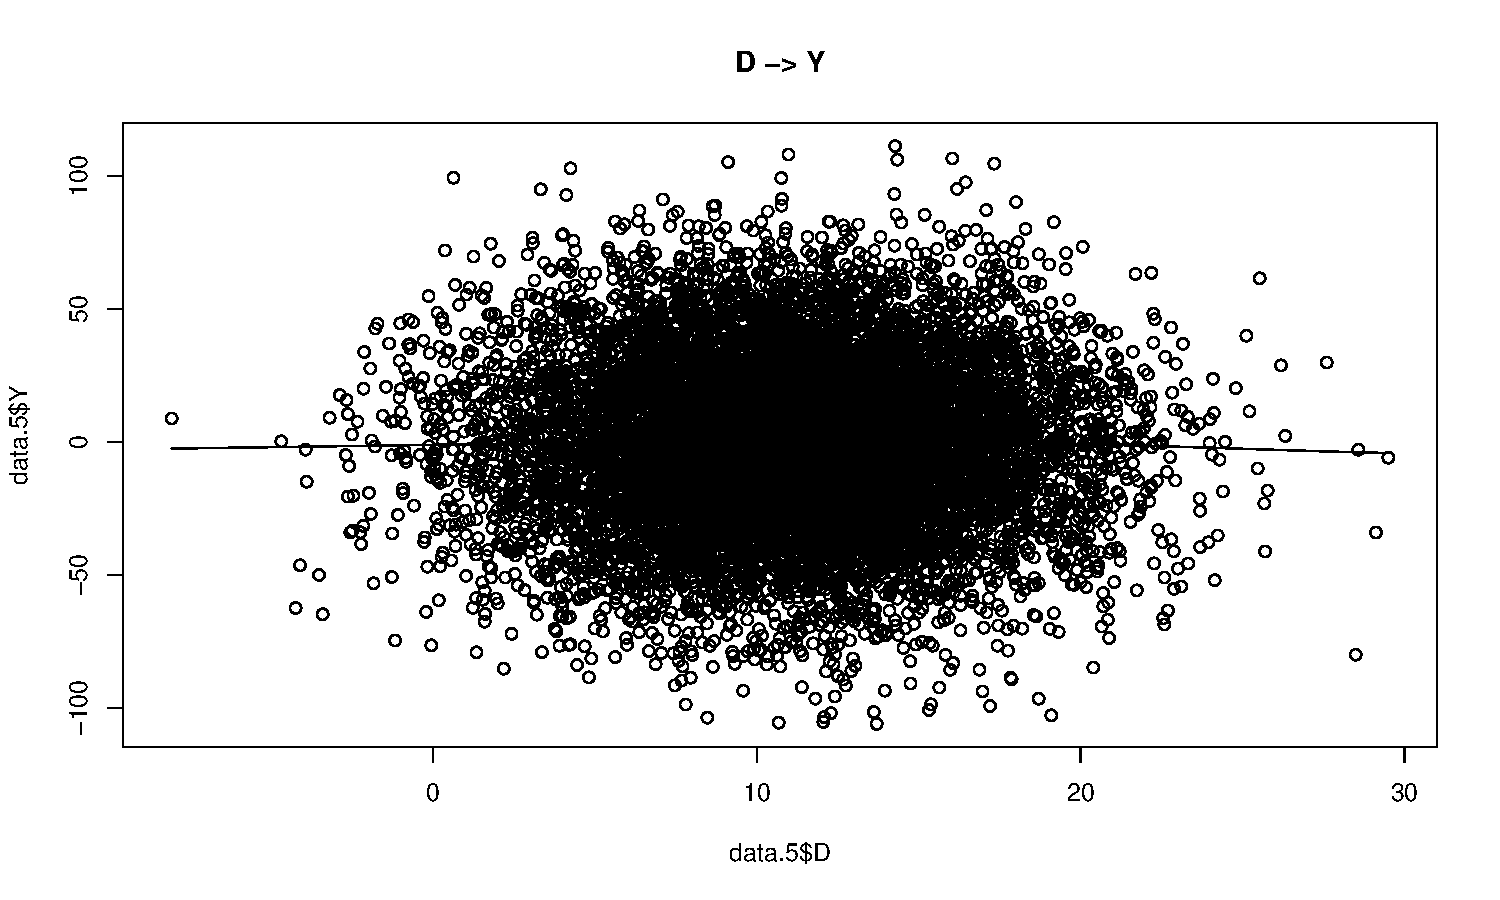
\includegraphics[width=\maxwidth]{figure/ExamplesVScatterplot-1} 
\end{knitrout}
\end{figure}
\end{frame}


\begin{frame}[fragile]{DAG Examples V: Regression result, NaivE}
% latex table generated in R 4.2.1 by xtable 1.8-4 package
% Fri Dec 16 17:22:33 2022
\begin{table}[ht]
\centering
\begingroup\small
\begin{tabular}{rrrrr}
  \hline
 & Estimate & Std. Error & t value & Pr($>$$|$t$|$) \\ 
  \hline
(Intercept) & 0.0195 & 0.8189 & 0.02 & 0.9810 \\ 
  D & -0.0488 & 0.0686 & -0.71 & 0.4769 \\ 
   \hline
\end{tabular}
\endgroup
\caption{Regression: lm(Y \textasciitilde ~D)} 
\end{table}
% latex table generated in R 4.2.1 by xtable 1.8-4 package
% Fri Dec 16 17:22:33 2022
\begin{table}[ht]
\centering
\begingroup\small
\begin{tabular}{rrr}
  \hline
 & 2.5 \% & 97.5 \% \\ 
  \hline
D & -0.18 & 0.09 \\ 
   \hline
\end{tabular}
\endgroup
\caption{95-Percent confidence interval: lm(Y \textasciitilde ~D)} 
\end{table}

\end{frame}

\begin{frame}[fragile]{DAG Examples V: Regression result, CIA I}
\textbf{Usage of Z1 to satisfy CIA}
% latex table generated in R 4.2.1 by xtable 1.8-4 package
% Fri Dec 16 17:22:33 2022
\begin{table}[ht]
\centering
\begingroup\small
\begin{tabular}{rrrrr}
  \hline
 & Estimate & Std. Error & t value & Pr($>$$|$t$|$) \\ 
  \hline
(Intercept) & -8.3448 & 0.8464 & -9.86 & 0.0000 \\ 
  D & 2.0501 & 0.1010 & 20.29 & 0.0000 \\ 
  C1 & -3.6986 & 0.1346 & -27.47 & 0.0000 \\ 
   \hline
\end{tabular}
\endgroup
\caption{Regression: lm(Y \textasciitilde ~D + C1)} 
\end{table}
% latex table generated in R 4.2.1 by xtable 1.8-4 package
% Fri Dec 16 17:22:33 2022
\begin{table}[ht]
\centering
\begingroup\small
\begin{tabular}{rrr}
  \hline
 & 2.5 \% & 97.5 \% \\ 
  \hline
D & 1.85 & 2.25 \\ 
   \hline
\end{tabular}
\endgroup
\caption{95-Percent confidence interval: lm(Y \textasciitilde ~D + C1)} 
\end{table}

\end{frame}

\begin{frame}[fragile]{DAG Examples V: Regression result, CIA II}
\textbf{Usage of Z2 to satisfy CIA}
% latex table generated in R 4.2.1 by xtable 1.8-4 package
% Fri Dec 16 17:22:33 2022
\begin{table}[ht]
\centering
\begingroup\small
\begin{tabular}{rrrrr}
  \hline
 & Estimate & Std. Error & t value & Pr($>$$|$t$|$) \\ 
  \hline
(Intercept) & -5.5728 & 0.7907 & -7.05 & 0.0000 \\ 
  D & 2.0116 & 0.0880 & 22.85 & 0.0000 \\ 
  C2 & -2.4464 & 0.0708 & -34.58 & 0.0000 \\ 
   \hline
\end{tabular}
\endgroup
\caption{Regression: lm(Y \textasciitilde ~D + C2)} 
\end{table}
% latex table generated in R 4.2.1 by xtable 1.8-4 package
% Fri Dec 16 17:22:33 2022
\begin{table}[ht]
\centering
\begingroup\small
\begin{tabular}{rrr}
  \hline
 & 2.5 \% & 97.5 \% \\ 
  \hline
D & 1.84 & 2.18 \\ 
   \hline
\end{tabular}
\endgroup
\caption{95-Percent confidence interval: lm(Y \textasciitilde ~D + C2)} 
\end{table}

\end{frame}

\begin{frame}[fragile]{DAG Examples V: Regression result, CIA III}
\textbf{Usage of Z3 to satisfy CIA}
% latex table generated in R 4.2.1 by xtable 1.8-4 package
% Fri Dec 16 17:22:33 2022
\begin{table}[ht]
\centering
\begingroup\small
\begin{tabular}{rrrrr}
  \hline
 & Estimate & Std. Error & t value & Pr($>$$|$t$|$) \\ 
  \hline
(Intercept) & -0.7023 & 0.8021 & -0.88 & 0.3813 \\ 
  D & 1.9977 & 0.0862 & 23.18 & 0.0000 \\ 
  C3 & -1.4751 & 0.0385 & -38.33 & 0.0000 \\ 
  C4 & -0.9925 & 0.0732 & -13.56 & 0.0000 \\ 
   \hline
\end{tabular}
\endgroup
\caption{Regression: lm(Y \textasciitilde ~D + C3 + C4)} 
\end{table}
% latex table generated in R 4.2.1 by xtable 1.8-4 package
% Fri Dec 16 17:22:33 2022
\begin{table}[ht]
\centering
\begingroup\small
\begin{tabular}{rrr}
  \hline
 & 2.5 \% & 97.5 \% \\ 
  \hline
D & 1.83 & 2.17 \\ 
   \hline
\end{tabular}
\endgroup
\caption{95-Percent confidence interval: lm(Y \textasciitilde ~D + C3 + C4)} 
\end{table}

\end{frame}



%------------------------------------------------------%
%--------------------- DAG VI -------------------------%
%------------------------------------------------------%

\begin{frame}{DAG Examples VI}
\\[1em]
\begin{figure}
\centering
\includegraphics[width=0.6\textwidth]{Graphics/6.TwoBack-doorpaths-Covered(missings).png}
\end{figure}
Question:
\begin{enumerate}
\item What is the causal path of interest?
\item What is/are the back-door path(s)? Are they open? How to block them?
\end{enumerate}
\\[1em]
$\rightarrow$ Is the result of the naive estimator the true causal effect?
\end{frame}


\begin{frame}{DAG Examples VI: Paths}
\begin{figure}
\includegraphics[width=0.5\textwidth]{{Graphics/6.TwoBack-doorpaths-Covered(missings).png}}
\end{figure}
\textbf{Paths:}
\begin{itemize}
\item Causal path: D $\rightarrow$ Y
\item 1. Back-door path: D $\leftarrow$ C\textsubscript{1} $\rightarrow$ C\textsubscript{2} $\rightarrow$ C\textsubscript{3} $\rightarrow$ Y
\item 2. Back-door path: D $\leftarrow$ C\textsubscript{1} $\rightarrow$ C\textsubscript{2} $\rightarrow$ C\textsubscript{4} $\rightarrow$ Y
\end{itemize}

\textbf{CIA satisfaction:}
\begin{itemize}
\item Only Z3 = \{C\textsubscript{3}, C\textsubscript{4}\} can be used because it is observed
\end{itemize}
\end{frame}


%------------------------------------------------------%
%--------------------- DAG VII ------------------------%
%------------------------------------------------------%

\begin{frame}{DAG Examples VII}
\\[1em]
\begin{figure}
\centering
\includegraphics[width=0.6\textwidth]{Graphics/6.TwoBack-doorpaths-Covered(moremissings).png}
\end{figure}
Question:
\begin{enumerate}
\item What is the causal path of interest?
\item What is/are the back-door path(s)? Are they open? How to block them?
\end{enumerate}
\\[1em]
$\rightarrow$ Is the result of the naive estimator the true causal effect?
\end{frame}


\begin{frame}{DAG Examples VII: Paths}
\begin{figure}
\includegraphics[width=0.5\textwidth]{{Graphics/6.TwoBack-doorpaths-Covered(moremissings).png}}
\end{figure}
\textbf{Paths:}
\begin{itemize}
\item Causal path: D $\rightarrow$ Y
\item 1. Back-door path: D $\leftarrow$ C\textsubscript{1} $\rightarrow$ C\textsubscript{2} $\rightarrow$ C\textsubscript{3} $\rightarrow$ Y
\item 2. Back-door path: D $\leftarrow$ C\textsubscript{1} $\rightarrow$ C\textsubscript{2} $\rightarrow$ C\textsubscript{4} $\rightarrow$ Y
\end{itemize}

\textbf{CIA satisfaction:}
\begin{itemize}
\item Not all back-door paths can be closed
\item CIA is only partially met by Z4 = \{C\textsubscript{4}\}
\item The estimate will contain a bias despite the closing of one back door path
\item The bias is induced by the back-door path that is still open
\end{itemize}
\end{frame}


\begin{frame}[fragile]{DAG Examples VII: Regression result, NaivE}
% latex table generated in R 4.2.1 by xtable 1.8-4 package
% Fri Dec 16 17:22:33 2022
\begin{table}[ht]
\centering
\begingroup\small
\begin{tabular}{rrrrr}
  \hline
 & Estimate & Std. Error & t value & Pr($>$$|$t$|$) \\ 
  \hline
(Intercept) & 0.0195 & 0.8189 & 0.02 & 0.9810 \\ 
  D & -0.0488 & 0.0686 & -0.71 & 0.4769 \\ 
   \hline
\end{tabular}
\endgroup
\caption{Regression: lm(Y \textasciitilde ~D)} 
\end{table}
% latex table generated in R 4.2.1 by xtable 1.8-4 package
% Fri Dec 16 17:22:33 2022
\begin{table}[ht]
\centering
\begingroup\small
\begin{tabular}{rrr}
  \hline
 & 2.5 \% & 97.5 \% \\ 
  \hline
D & -0.18 & 0.09 \\ 
   \hline
\end{tabular}
\endgroup
\caption{95-Percent confidence interval: lm(Y \textasciitilde ~D)} 
\end{table}

\end{frame}

\begin{frame}[fragile]{DAG Examples VII: Regression result, CIA I}
\textbf{Usage of Z4 to partially satisfy CIA}
% latex table generated in R 4.2.1 by xtable 1.8-4 package
% Fri Dec 16 17:22:33 2022
\begin{table}[ht]
\centering
\begingroup\small
\begin{tabular}{rrrrr}
  \hline
 & Estimate & Std. Error & t value & Pr($>$$|$t$|$) \\ 
  \hline
(Intercept) & -0.9820 & 0.8590 & -1.14 & 0.2529 \\ 
  D & 0.0676 & 0.0749 & 0.90 & 0.3666 \\ 
  C4 & 0.2687 & 0.0700 & 3.84 & 0.0001 \\ 
   \hline
\end{tabular}
\endgroup
\caption{Regression: lm(Y \textasciitilde ~D + C3)} 
\end{table}
% latex table generated in R 4.2.1 by xtable 1.8-4 package
% Fri Dec 16 17:22:33 2022
\begin{table}[ht]
\centering
\begingroup\small
\begin{tabular}{rrr}
  \hline
 & 2.5 \% & 97.5 \% \\ 
  \hline
D & -0.08 & 0.21 \\ 
   \hline
\end{tabular}
\endgroup
\caption{95-Percent confidence interval: lm(Y \textasciitilde ~D + C4)} 
\end{table}

\end{frame}


%------------------------------------------------------%
%--------------------- DAG VIII -----------------------%
%------------------------------------------------------%

\begin{frame}{DAG Examples VIII}
\\[1em]
\begin{figure}
\centering
\includegraphics[width=0.6\textwidth]{Graphics/7.Collider.png}
\end{figure}
Question:
\begin{enumerate}
\item What is the causal path of interest?
\item What is/are the back-door path(s)? Are they open? How to block them?
\end{enumerate}
\\[1em]
$\rightarrow$ Is the result of the naive estimator the true causal effect?
\end{frame}


\begin{frame}{DAG Examples VIII: Paths}
\begin{figure}
\includegraphics[width=0.5\textwidth]{{Graphics/7.Collider.png}}
\end{figure}
\textbf{Paths:}
\begin{itemize}
\item Causal path: D $\rightarrow$ Y
\item 1. Back-door path: D $\leftarrow$ C\textsubscript{1} $\rightarrow$ C\textsubscript{2} $\leftarrow$ C\textsubscript{3} $\rightarrow$ Y
\end{itemize}

\textbf{CIA satisfaction:}
\begin{itemize}
\item Automatically satisfied because of the collier on back-door path 
\end{itemize}
\end{frame}


\begin{frame}{DAG Examples VIII: Scatterplot}
\begin{figure}
\begin{knitrout}
\definecolor{shadecolor}{rgb}{0.969, 0.969, 0.969}\color{fgcolor}
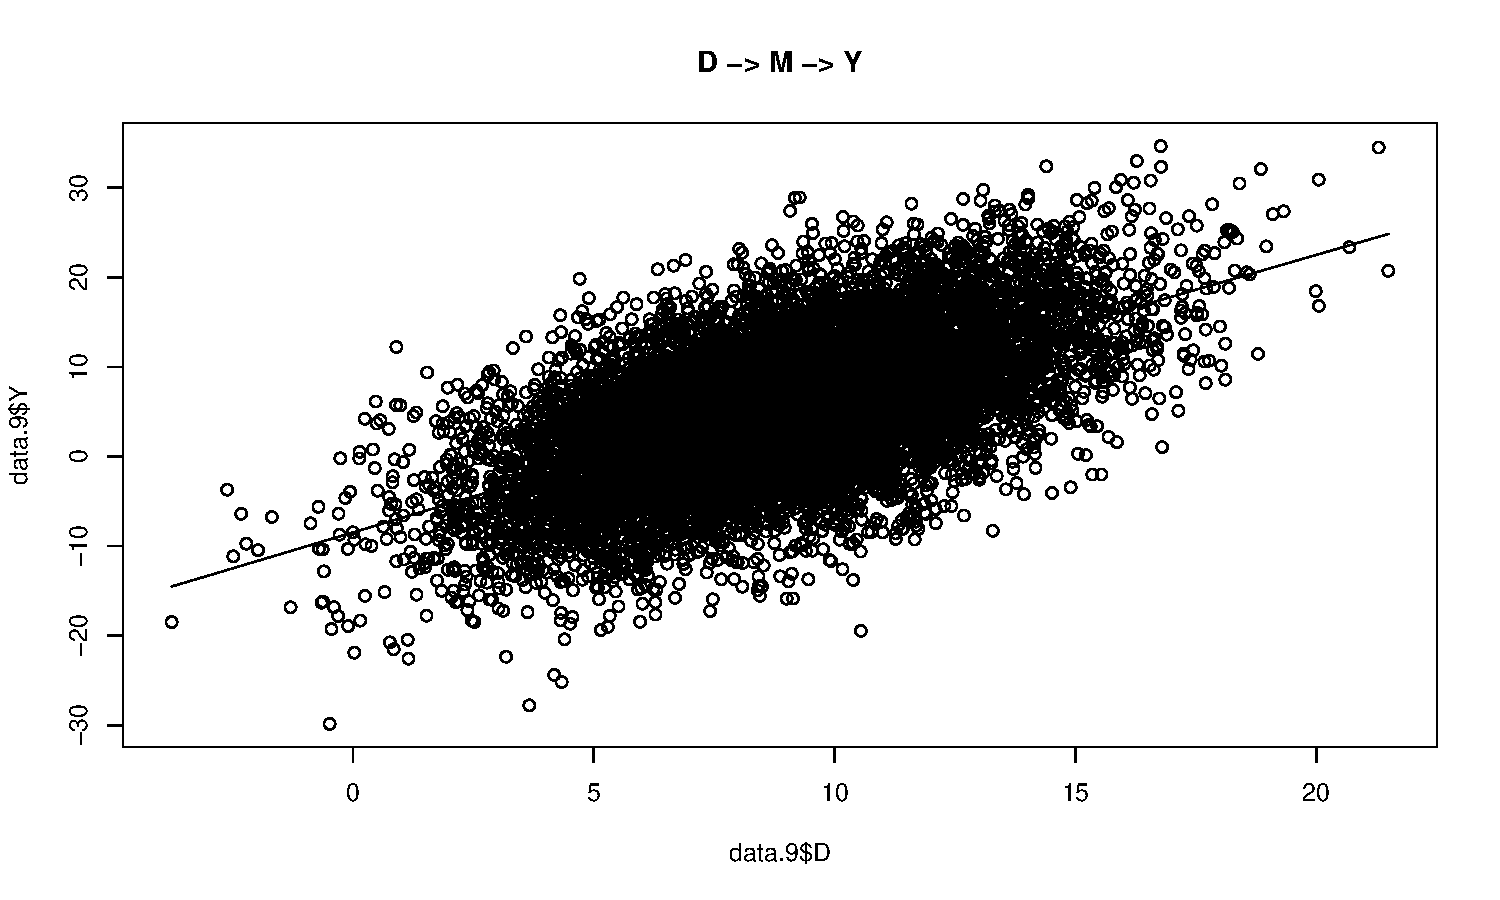
\includegraphics[width=\maxwidth]{figure/ExamplesVIIIScatterplot-1} 
\end{knitrout}
\end{figure}
\end{frame}


\begin{frame}[fragile]{DAG Examples VIII: Regression result, NaivE}
% latex table generated in R 4.2.1 by xtable 1.8-4 package
% Fri Dec 16 17:22:34 2022
\begin{table}[ht]
\centering
\begingroup\small
\begin{tabular}{rrrrr}
  \hline
 & Estimate & Std. Error & t value & Pr($>$$|$t$|$) \\ 
  \hline
(Intercept) & -8.2163 & 0.1962 & -41.88 & 0.0000 \\ 
  D & 1.5197 & 0.0207 & 73.57 & 0.0000 \\ 
   \hline
\end{tabular}
\endgroup
\caption{Regression: lm(Y \textasciitilde ~D)} 
\end{table}
% latex table generated in R 4.2.1 by xtable 1.8-4 package
% Fri Dec 16 17:22:34 2022
\begin{table}[ht]
\centering
\begingroup\small
\begin{tabular}{rrr}
  \hline
 & 2.5 \% & 97.5 \% \\ 
  \hline
D & 1.48 & 1.56 \\ 
   \hline
\end{tabular}
\endgroup
\caption{95-Percent confidence interval: lm(Y \textasciitilde ~D)} 
\end{table}

\end{frame}

\begin{frame}[fragile]{DAG Examples VIII: Regression result, wrong control}
\textbf{Usage of Z1 to satisfy CIA}
% latex table generated in R 4.2.1 by xtable 1.8-4 package
% Fri Dec 16 17:22:34 2022
\begin{table}[ht]
\centering
\begingroup\small
\begin{tabular}{rrrrr}
  \hline
 & Estimate & Std. Error & t value & Pr($>$$|$t$|$) \\ 
  \hline
(Intercept) & -6.2713 & 0.1713 & -36.62 & 0.0000 \\ 
  D & 1.8519 & 0.0185 & 99.84 & 0.0000 \\ 
  C2 & 0.8255 & 0.0137 & 60.09 & 0.0000 \\ 
   \hline
\end{tabular}
\endgroup
\caption{Regression: lm(Y \textasciitilde ~D + C1)} 
\end{table}
% latex table generated in R 4.2.1 by xtable 1.8-4 package
% Fri Dec 16 17:22:34 2022
\begin{table}[ht]
\centering
\begingroup\small
\begin{tabular}{rrr}
  \hline
 & 2.5 \% & 97.5 \% \\ 
  \hline
D & 1.82 & 1.89 \\ 
   \hline
\end{tabular}
\endgroup
\caption{95-Percent confidence interval: lm(Y \textasciitilde ~D + C2)} 
\end{table}

\end{frame}


%-------------------------------------------------------------%
%---- Experimental vs. non-experimental designs --------------%
%-------------------------------------------------------------%

\section{Experimental vs. non-experimental designs} % Wichtig für Inhaltsverzeichnis

\begin{frame}{Experimental designs}
  \begin{itemize}
  \item The central feature of \textbf{experimental designs} is the random distribution of the observations (e.g. test subjects) between a treatment group and a control group (\textit{randomization})
  \item Due to the randomization, these are often seen as an ideal design for drawing causal inferences because the \textbf{IA is automatically satisfied}
  \item \textbf{Problem:} Often experimental designs cannot be implemented due to \textit{practical and ethical problems}
  \item In addition, experiments can have problems \textit{internal and external validity}
  \end{itemize}
\end{frame}


\begin{frame}{Non-experimental designs}
  \begin{itemize}
    \item Frequent use in the social sciences of non-experimental methods of causal analysis based on observational data
    \item Data sources are e.g. general population surveys such as ALLBUS, SOEP or ESS
    \item \textbf{Problems:}
      \begin{itemize}  
        \item Non-random selection
        \item CIA/IA needs to be satisfied
      \end{itemize}
  \end{itemize}
\end{frame}

\begin{frame}{(Temporal) dataset structure I}
\textbf{Cross-sectional data}
  \begin{itemize}
    \item No time dimension in the outcome variable (Y): measurement only once at time t1
    \item Treatment variable (D) is also recorded at the same point in time t1 ... \\[0.5em]
      \begin{itemize}  
        \item (A) ... but based on theoretical reasons it can be assumed to take place earlier, even if the measurement relates to time t1. (\textit{Example: D:father's level of education, Y:respondent's income}) \\[0.5em]
        \item (B) ... but can, as a retrospective question, relate to an earlier point in time t0 (or period)
      \end{itemize}
  \end{itemize}
\end{frame}


\begin{frame}{(Temporal) dataset structure II}
\textbf{Longitudinal data}
  \begin{itemize}
    \item At least two measurements of the Y variable in time to capture changes in Y.
    \item Additional condition for the implementation of a "fixed-effect" logic: \\
    At least one measurement of the Y variable must relate to a point in time before the treatment (= change over time in the D variable of interest) and at least one measurement of the Y variable must relate to a point in time after the treatment
  \end{itemize}
\end{frame}



%Aufgabe zur nächsten Sitzung
\begin{frame}{Task for the next meeting}
\begin{itemize}
  \item Search for possible confounders of the chosen connections. \\[1em]
  \item Include this in the already created document. \\[1em]
  \item Inclusion of the confounder(s) in the regression analysis as control variable(s). \\[1em]
\end{itemize}
\end{frame} 



%Noch Fragen
\begin{frame}

\center{Do you still have any questions?}
  
\end{frame} 


\end{document}
